%
% Modified by Megan Patnott
% Last Change: Jan 18, 2013
%
%%%%%%%%%%%%%%%%%%%%%%%%%%%%%%%%%%%%%%%%%%%%%%%%%%%%%%%%%%%%%%%%%%%%%%%%
%
% Modified version of the sample_ndthesis.tex
% by Sameer Vijay
% Last Change: Wed Jul 27 2005 14:00 CEST
%
%%%%%%%%%%%%%%%%%%%%%%%%%%%%%%%%%%%%%%%%%%%%%%%%%%%%%%%%%%%%%%%%%%%%%%%%
%
% Sample Notre Dame Thesis/Dissertation
% Using Donald Peterson's ndthesis classfile
%
% Written by Jeff Squyres and Don Peterson
%
% Provided by the Information Technology Committee of
%   the Graduate Student Union
%   http://www.gsu.nd.edu/
%
% Nothing in this document is serious except the format.  :-)
%
%%%%%%%%%%%%%%%%%%%%%%%%%%%%%%%%%%%%%%%%%%%%%%%%%%%%%%%%%%%%%%%%%%%%%%%%
% This is *not* a substitute for the documentation, which is included
% as a pdf file in the standard distribution, and can be obatined from
% the dtx file in the advanced distribution.
%%%%%%%%%%%%%%%%%%%%%%%%%%%%%%%%%%%%%%%%%%%%%%%%%%%%%%%%%%%%%%%%%%%%%%%%
%
% You should *also* have a ND formatting guide to ensure that you have
% all the relevant parts, put the captions in the right place, etc.
% Just because you have this wonderful style classfile doesn't mean
% that it removes *all* the formatting onus from you.  :-)
% Although be warned that the Graduate School has been known to let
% their official formatting guide get out of date. When in doubt,
% the Microsoft Word example seemed to be the only thing kept
% consistently up-to-date in 2013, and is probably the safest thing
% to consult.
%
% You should break all of this stuff up into separate files
% (at the very least, one chapter per file) and use the \include
% command, as has been done here for chapters 1 and 2 and the appendix.
% There is also an \input command, but \include is more commonly used to
% import chapters in books and dissertations. For the differences between these
% two commands, see, e.g., 
% http://web.science.mq.edu.au/~rdale/resources/writingnotes/latexstruct.html
% or http://tex.stackexchange.com/questions/246/when-should-i-use-input-vs-include.
%
% If you compile from the command line, note that you should also have 
% a good Makefile; one that invokes LaTeX as many times as necessary 
% (up to 4) and bibtex if necessary.
%
% If you use an editor that allows you to compile from within the
% program, note that you will need to compile up to four times. Also,
% we recommend that you use pdflatex (sometimes displayed as
% LaTeX => PDF) to compile directly to pdf.
%
% If you have any suggestions, comments, questions, please send e-mail
% to: dteditor@nd.edu
%
%%%%%%%%%%%%%%%%%%%%%%%%%%%%%%%%%%%%%%%%%%%%%%%%%%%%%%%%%%%%%%%%%%%%%%%%

\documentclass[draft,numrefs,sort&compress]{nddiss2e}
% One of the options draft, review, final must be chosen.
% One of the options textrefs or numrefs should be chosen
% to specify if you want numerical or ``author-date''
% style citations.
% Other available options are:
% 10pt/11pt/12pt (available with draft only)
% twoadvisors
% noinfo (should be used when you compile the final time
%         for formal submission)
% sort (sorts multiple citations in the order that they're
%       listed in the bibliography)
% compress (compresses numerical citations, e.g. [1,2,3]
%           becomes [1-3]; has no effect when used with
%           the textrefs option)
% sort&compress (sorts and compresses numerical citations;
%           is identical to sort when used with textrefs)

\usepackage{graphicx}% Include figure files
\usepackage{amssymb}
\usepackage{amsmath}
\usepackage{mhchem}
\usepackage{revsymb}
\usepackage{bm}
\usepackage{realboxes}
\usepackage{morefloats}
\usepackage[flushleft]{threeparttable} 
\usepackage{rotating}
\usepackage{subfig}
\usepackage{enumitem}
\usepackage{gensymb}
\usepackage{graphicx}
\usepackage{topcapt}
\usepackage{booktabs}
\usepackage{commath}
\usepackage{units}
\usepackage{makecell}
\usepackage{adjustbox}
%\usepackage{amsfonts}


\begin{document}

\frontmatter % All the items before the first chapter go in ``frontmatter''

% Titles may be 1-4 lines long. If your title is longer than 4 lines,
% the class file may have difficulty formatting the title page.
% Line-breaks in the title have to be protected with `\protect`.
\title{$^{14}$N$\left( p,\gamma \right) ^{15}$O}
% TITLE OF WORK. It must be in all caps, and ensuring this is your
 % responsiblity.
\author{Bryce Alan Frentz}
\work{Dissertation} % or \work{Thesis}
\degaward{Doctor of Philosophy} % or 
%\degaward{Master of Science \\ in \\ Subject}
\advisor{Ani Aprahamian}
\department{Physics}

\maketitle
%%%%%%%%%%%%%%%%%%%%%%%%%%%%%%%%%%%%%%%%%%%%%%%%%%%%%%%%%%%%%%%%%%%%%%%%
%
% Front stuff
%
%%%%%%%%%%%%%%%%%%%%%%%%%%%%%%%%%%%%%%%%%%%%%%%%%%%%%%%%%%%%%%%%%%%%%%%%

% You must either set the copyright information or put your work in the public domain.
\copyrightholder{Bryce Frentz} % See template or documentation for
\copyrightyear{2019}           % other copyright options.
\copyrightlicense{CC-BY-4.0}
\makecopyright

% An abstract is optional for a mster's thesis, and required for a doctoral dissertation.
\begin{abstract}
  
  $^{14}$N$\left( p,\gamma \right) ^{15}$O \\
  
  What do you even put in an abstract for a thesis? Seems a little ridiculous...
  
\end{abstract}

% A dedication is optional.
\renewcommand{\dedicationname}{NEW DEDICATION NAME}

\begin{dedication}
  To .... probably nobody
\end{dedication}

% These are required, and must be in this order.
\tableofcontents
\listoffigures
\listoftables

% A preface is optional.
\begin{preface}
  It is often said that there are few places left to be discovered or explored. That's only true on the human scale. Using a magnifying glass, microscope, telescope or any other number of devices allows us to transcend our scale.
  
  Taken in isolation, different structures are like characters in a story. Each contributes something to the otherall shape. Sometimes one or a handful of characters will dominate the story, but it is is only when put together that they fully explain why the world behaves the way it does.
  
  The stars twinkle their cryptic morse code and nuclear physics is one of the best keys to their cypher.
  
  When numbers acquire the significance of language they acquire the power to do all of the things that language can do. Describe power history success failure victory defeat character grace to become fiction, drama, and poetry. 
  
  Discovering stable relationships in a seemingly unstable world.
\end{preface}

% It's hard to tell from the information available from the Graduate
% School in Spring 2013 whether or not an acknowledgements section is optional.
\begin{acknowledge}
  I would like to acknowledge ...
\end{acknowledge}

% A symbols section is optional.
\begin{symbols}
  \sym{\mathcal{F}}{sighting frequency of Gnus about campus}
  \sym{p}{student population}
  \sym{f}{type of food available}
  \sym{d}{day of week}
  \sym{c}{speed of light}
  \sym{m}{mass}
  \sym{e}{elementary charge}
  \sym{a,b}{miscellaneous constants}  
  \sym{E}{energy}  
\end{symbols}

\mainmatter
% Place the text body here.
%\include{chapter-one}
%Begin each chapter with \chapter{Title}. Both the thesis title and
%chapter titles should match in style.

%
% An unnumbered chapter (features)
%
\unnumchapter{Features of Formatting in This Example File}
% The \unnumchapter command allows you to include an unnumbered chapter as part of
% the main text before Chapter 1. It will appear in your table of contents, and you
% should have at most one such chapter (although nothing in the class file will
% prevent you from creating more).

% The usual \cite{} command is also available, and should work as expected.
This \verb+chapter+ has been added to the original sample file to highlight the
various features with the formatting that conforms to the Graduate school
guidelines --- whether obtained due to the use of \nddiss\/ class file or just
plain good practice.
\begin{itemize}
\item An important note on line-breaks via \verb+\\+ in titles: the
  titles of the thesis as well as chapters and table captions use
  \verb+\MakeTextUppercase{}+ from the \verb+textcase+ package.  Due
  to the nature of the \verb+center+ environment, any line-breaks
  introduced in titles and captions should be protected, as in
  \verb+\protect\\+.
  To preserve the case in titles and captions, use, e.g.,
  \verb+\NoCaseChange{Gnus}+.
\item In the \emph{dedication}, the title name has been modified. So, you know
how to and that it can be done.
\item The entries in the \emph{List of figures} and \emph{List of Tables} are
single-spaced themselves but are double-spaced from the other.
\item The table captions are not in all CAPS as well for the reason mentioned
above.
\item Appropriate space is left between the \verb+Table xx+ and its
corresponding caption (which is double-spaced itself) as in table \ref{tbl:bogus1}.
\item Tables look much better without the vertical lines (good practice).
\item There is double-spacing between the table entries but single-spacing
within the entry.
\item The chapter (see Chapter \ref{chap:golfing}) or section titles are
double-spaced as mentioned in the guidelines.
\item There is a \verb+subsubsection+ present (eg. section \ref{sec:data}) and
is properly formatted in the TOC.
\item Sections deeper than \verb+subsubsection+ should not appear in the TOC.
\item Table \ref{tbl:defs} is an example of the use of \textsf{landscape}
environment in which a normal table is formatted in a \emph{landscape} mode.
\item The \textsf{longtable} environment is used in Tables \ref{tbl:votes} and
\ref{tbl:rotated-rankings}, in normal and \verb+landscape+ mode, respectively. The
table captions are formatted properly in both cases.
\item In the table \ref{tbl:votes}, the \verb+footnote+ in the table header 
does not appear at all. This is not an error of the \nddiss\/ class but of the
\textsf{longtable} package.
\item An example of citing a website is shown in the bibliography (see
\citep{gairley2000}) which is formatted using the \verb+nddiss2e.bst+
citation style file.
\item A bit of information on the \nddiss\/ class file and the typesetting program
used is included in a box on the last page of the thesis.
\item Footnotes should space properly.
\item Items in \verb+itemize+, \verb+enumerate+, and \verb+description+ environment
should automatically single-space within an item, but double space between items.
\end{itemize}

%
% Chapter 1
%

%
% Modified by Megan Patnott
% Last Change: Jan 18, 2013
%
%%%%%%%%%%%%%%%%%%%%%%%%%%%%%%%%%%%%%%%%%%%%%%%%%%%%%%%%%%%%%%%%%%%%%%%%
%
% Modified by Sameer Vijay
% Last Change: Tue Jul 26 2005 13:00 CEST
%
%%%%%%%%%%%%%%%%%%%%%%%%%%%%%%%%%%%%%%%%%%%%%%%%%%%%%%%%%%%%%%%%%%%%%%%%
%
% Sample Notre Dame Thesis/Dissertation
% Using Donald Peterson's ndthesis classfile
%
% Written by Jeff Squyres and Don Peterson
%
% Provided by the Information Technology Committee of
%   the Graduate Student Union
%   http://www.gsu.nd.edu/
%
% Nothing in this document is serious except the format.  :-)
%
% If you have any suggestions, comments, questions, please send e-mail
% to: ndthesis@gsu.nd.edu
%
%%%%%%%%%%%%%%%%%%%%%%%%%%%%%%%%%%%%%%%%%%%%%%%%%%%%%%%%%%%%%%%%%%%%%%%%


%
% Chapter 1
%

\chapter{Introduction}
\label{chap: introduction}

\section{Overview}
\label{sec: Nuclear astrophysics overview}

\subsection{General overview}

Nuclear physics data, in both the forms of theoretical predictions and experimental results, is an ever richer trove of information useful in solving many astrophysical problems. The partnership between the fields of nuclear physics and astrophysics was actually born in the early days of nuclear physics when Sir Arthur Eddington postulated that recent laboratory discoveries could explain the energy generation of the sun and stars cite{IliadisBook}. Therefore, developments in one area naturally link to increased knowledge in the other - a scientific point and counterpoint. It follows naturally that many astrophysical phenomena are governed by nuclear physics. So it is through this study of the microscopic aspects of the universe that we also elucidate its behavior in the grandest scales imaginable. 

The general goals of the field of nuclear astrophysics are as follows:
\begin{itemize}
\item to understand the processes by which the chemical elements were formed
\item to understand the mechanism(s) responsible for the the relative abundances between the chemical elements
\item to understand the energy generation during each phase of stellar evolution.
\end{itemize}

\noindent Crucially, stellar evolution is cyclic: stars are born, evolve, and ultimately die, seeding the interstellar medium with the collective material they've created over their life in order to form the building blocks for the next stellar generation. As each of the different stellar phases are guided by the underlying nuclear physics, investigations into these questions provide a rich ink between humans and our place in the cosmos. 

The synthesis of the chemical elements we see began with the universe as the Big Bang created hydrogen, helium, and trace amounts of lithium cite{Alpher1948}. Shortly after the Big Bang, the temperature and density of the Universe dropped too low for any significant nuclear fusion to occur and overcome the mass 5 and mass 8 barriers. This was the end of Big Bang Nucleosynthesis (BBN), as after this point, the elemental abundances were nearly stable, with the only changes coming from the radioactive decay of $^{3}$He $\rightarrow$ $t$ and $^{7}$Be $\rightarrow$ $^{7}$Li cite{Fields2011}.

\begin{figure}
\label{fig: abundances}
\caption{The current solar abundance pattern. }
\end{figure}

From this point, generations of stellar evolution created nearly all other elements, leading to the currently observed elemental abundance distribution, shown in Figure \ref{fig: abundances}. The synthesis of elements heavier than BBN products, commonly referred to as "metals," began with the formation of the first stars. Cold gas clouds, composed primarily the BBN products of hydrogen and helium (and metals in subsequent stellar generations), coalesce under their mutual gravitational attraction, converting their gravitational potential energy to heat -- increasing their pressure, density, and temperature. Upon passing a critical threshold for these physical quantities, typically temperatures $>$1 MK, thermonuclear fusion reactions begin in the core cite{RyanNortonBook}. This transition marks the "birth" of a star, having reached a point where nuclear reactions provide a sufficient heat source to balance energy losses from radiation. 


\subsection{Stellar evolution}

Every star is unique and their intrinsic quantities when forming, such as mass or initial abundance distribution, prescribe the nuclear reactions that can occur throughout their lifetimes. Despite their differences, correlations emerge in studies of their observational properties , like luminosity, mass distribution, temperature, color, etc. The most evident patterns appeared when classifying stars by luminosity (or magnitude) vs temperature (or color), named the \textit{Hertzsprung-Russel} (HR) diagram cite{CarrollOstlieBook, IliadisBook, RyanNortonBook}, distilling the most important relationship between stellar properties. An example HR diagram for stars in the solar neighborhood is displayed in Figure \ref{fig: HR_diagram}. Since HR diagrams represent a snapshot of the evolutionary tack of a set of stars, the most densely populated areas of such plots are those in which individual stars necessarily spend most of their lives. Conversely, as there is a lower probability of observing a star in a short-lived phase, sparsely populated areas of HR diagrams detail such phases of stellar burning. 

The vast majority of stars lie on the diagonal band stretching from the upper left (hot, bright stars) to the lower right (cool, faint stars) of the diagram. This feature is called the main sequence. These stars support themselves through core hydrogen burning -- implying that stars spend most of their lives in this long period of quiescent hydrogen burning in the \textit{pp chains} and the CNO cycles, detailed in subsequent sections. Other prominent features of typical HR diagrams are the clusters of stars in the upper quadrants (very bright stars), commonly referred to as the giant branch, the lower left quandrant (hot, faint stars), where the white dwarf stars reside, and the lower right quadrant beyond the main sequence, occupied by brown dwarfs. Each classification corresponds to different nuclear reactions, with stars evolving off the main sequence being characterized by phases of burning of heavier elements, like helium or carbon. 

\begin{figure}
\label{fig: HR_diagram}
\caption{An example of a Herzprung-Russell diagram. The horizontal axis gives the temperature of the star while the vertical shows the stellar luminosities.}
\end{figure}

Any single star's evolutionary track will follow different paths depending on its initial mass cite{IliadisBook, RyanNortonBook}.  For cosmic objects of mass $\lesssim$ 0.08 M$_{\odot}$, where M$_{\odot}$ is the mass of the sun, core temperatures never rise high enough to sustain hydrogen fusion, and thus they evolve directly into brown dwarf stars. In the range of mass 0.08 M$_{\odot} \lesssim$ M $\lesssim$0.4 M$_{\odot}$, stars undergo core hydrogen fusion through the \textit{pp chains}, but do not reach temperatures sufficient to initiate helium burning after exhausting hydrogen in the core. Ultimately, stars in this classification become white dwarfs. The next mass grouping consists of Sun-like stars, with masses 0.4 M$_{\odot} \lesssim$ M $\lesssim$ 8.0 M$_{\odot}$, which evolve off the main sequence and continue growing and burning (both in the stellar core and shells in their stellar envelope). Such stars achieve temperatures high enough to create final abundance distribution composed of primarily carbon and oxygen in their core. After losing their stellar envelopes, these stars are carbon-oxygen white dwarfs. However, if such a star has a companion of sufficient mass, it will eventually explode in a type Ia supernova. Lastly, are stars of mass 8.0 M$_{\odot}$ $\lesssim$ M, which go through sequences of carbon, neon, oxygen, and silicon burning to produce a dominantly iron-nickel core. At this point, as the stars are more massive than the Chandrasekar limit, the gravitational attraction will exceed the support of elecron degeneracy pressure causing a core collapse (type II) supernova. Depending on the star's mass at this stage, it will become either a neutron star or black hole. While not the topic of this thesis, such explosive scenarios are currently an area of intense research as they are the location of many unresolved issues of nuclear astrophysics, including what the National Research Council identified in 2003 as one of the eleven greatest unanswered questions of the century, namely the origin of the elements heavier than iron cite{Turner2003}.


\subsection{Hydrogen Burning}

The lifetimes of stars along the main sequence vary drastically, from millions of years to trillions of years, depending on the star's properties when forming. Likewise, the dominant type of hydrogen burning that occurs during the main sequence phase is also highly dependent on stellar characteristics like mass and initial composition. Broadly, there are two sets of nuclear processes that comprise the hydrogen burning phases in stellar cores, the \textit{pp chains} and the CNO cycles, with each ultimately functions in a similar way, to convert four hydrogen nuclei to one helium nucleus, releasing $ \sim$26 MeV of energy cite{RolfsBook}. 

The \textit{pp chains} are the main energy generator in smaller stars with core temperatures below 20 MK cite{RyanNortonBook}, like the sun. There are three variations of the \textit{pp chains} (denoted ppI, ppII, and ppIII), shown below.

\begin{align*}
\underline{\mathrm{ppI}} & & \underline{\mathrm{ppII}} & &\underline{\mathrm{ppIII}}  & \\
p\left(p, e^{+} \nu \right) d & & p\left(p, e^{+} \nu \right) d & & p\left(p, e^{+} \nu \right) d \\
d\left(p, \gamma \right) \ce{^{3}He} & & d\left(p, \gamma \right) \ce{^{3}He} & & d\left(p, \gamma \right) \ce{^{3}He} \\ 
\ce{^{3}He} \left( \ce{^{3}He}, 2p \right) \ce{^{4}He} & & \ce{^{3}He} \left( \ce{^{4}He}, \gamma \right) \ce{^{7}Be} &  &  \ce{^{3}He} \left( \ce{^{4}He}, \gamma \right) \ce{^{7}Be}  \\
& & \ce{^{7}Be}  \left( e^{-} \nu \right) \ce{^{7}Li} & & \ce{^{7}Be} \left( p, \gamma \right) \ce{^{8}B} \\
& & \ce{^{7}Li} \left( p, \alpha \right) \ce{^{4}He} & & \ce{^{8}B} \left( e^{+} \nu \right) \ce{^{8}Be} \\
& & & & \ce{^{8}Be} \left( \alpha \right) \ce{^{4}He} 
\end{align*}

Between the three branches there are clear similarities and differences. The energy released between each of ppI, ppII, and ppIII are 26.20 MeV, 25.66 MeV, and 19.75 MeV, respectively, with the difference coming from the amount of energy carried away by the electrons, positrons, and neutrinos. Of these chains, ppI is the most prominent, occurring $\sim$ 85 \% of the time, where the remainder branches off as a $\ce{^{3}He}$ nucleus will fuse with a $\ce{^{4}He}$ nucleus, resulting in the ppII or ppIII chain, occurring $\sim$ 14.99 \% and $\sim$ 0.1 \% of the time, respectively cite{RyanNortonBook}. Regardless of the branching for the \textit{pp chains}, each starts with the $p\left(p, e^{+} \nu \right) d$ reaction. This reaction is governed purely by the weak interaction, and thus is about 20 orders of magnitude slower than those proceeding via the strong interaction cite{RolfsBook}, like the reactions in the chains that follow. Therefore, energy production, nucleosynthesis, and stellar evolution timescales for stars dominated by the \textit{pp chains} are restricted by the $p\left(p, e^{+} \nu \right) d$ reaction.

However, for most stars the CNO cycles are the dominant energy source. Stellar energy generation depends sensitively on the temperature in the star's core, which is closely tied to its mass. For stars of mass M $\gtrsim$ M$_{\odot}$, where cores contain carbon and oxygen seed nuclei and temperatures exceed 20 MK, the CNO cycles' energy production overtakes that of the \textit{pp chains}. Thus, the knowledge of the overall rate of this cycle is important for the study of their evolution. 

The CNO cycles are the collection of four similar energy producing cycles broadly characterized by their synthesis of helium from hydrogen with a carbon catalyst, seeded by earlier generations of stars. There are four CNO cycles, listed below with their relationships shown in Fig. \ref{fig: CNO-cycles}.

\begin{align*}
\underline{\mathrm{CNO1}} & & \underline{\mathrm{CNO2}} & &\underline{\mathrm{CNO3}}  & & \underline{\mathrm{CNO4}} & \\
\ce{^{12}C} \left( p, \gamma \right) \ce{^{13}N} & & \ce{^{14}N} \left( p, \gamma \right) \ce{^{15}O} & & \ce{^{15}N} \left( p, \gamma \right) \ce{^{16}O} & & \ce{^{16}O} \left( p, \gamma \right) \ce{^{17}F}\\
\ce{^{13}N} \left( \beta^{+} \nu \right) \ce{^{13}C} & & \ce{^{15}O} \left( \beta^{+} \nu \right) \ce{^{15}N} & & \ce{^{16}O} \left( p, \gamma \right) \ce{^{17}F} & & \ce{^{17}F} \left( \beta^{+} \nu \right) \ce{^{17}O} \\
\ce{^{13}C} \left( p, \gamma \right) \ce{^{14}N} & & \ce{^{15}N} \left( p, \gamma \right) \ce{^{16}O} & & \ce{^{17}F} \left( \beta^{+} \nu \right) \ce{^{17}O} & & \ce{^{17}O} \left( p, \gamma \right) \ce{^{18}F}\\
\ce{^{14}N} \left( p, \gamma \right) \ce{^{15}O} & & \ce{^{16}O} \left( p, \gamma \right) \ce{^{17}F} & & \ce{^{17}O} \left( p, \gamma \right) \ce{^{18}F} & & \ce{^{18}F} \left( \beta^{+} \nu \right) \ce{^{18}O} \\
\ce{^{15}O} \left( \beta^{+} \nu \right) \ce{^{15}N} & & \ce{^{17}F} \left( \beta^{+} \nu \right) \ce{^{17}O} & & \ce{^{18}F} \left( \beta^{+} \nu \right) \ce{^{18}O} & & \ce{^{18}O} \left( p, \gamma \right) \ce{^{19}F}\\
\ce{^{15}N} \left( p, \alpha \right) \ce{^{12}C} & & \ce{^{17}O} \left( p, \alpha \right) \ce{^{14}N} & & \ce{^{18}O} \left( p, \alpha \right) \ce{^{15}N} & & \ce{^{19}F} \left( p, \alpha \right) \ce{^{16}O}
\end{align*}

\noindent As with the \textit{pp chains}, the net result of each of the CNO cycles is the conversion of four protons into helium, releasing $\sim$ 26 MeV of energy in the process cite{RyanNortonBook}. Additionally, all of the heavier elements (carbon, nitrogen, oxygen, and fluorine) are only catalysts, with their overall abundance unchanged through the cycles while only the hydrogen is consumed. Therefore, this implies that the CNO cycles can occur even if the amount of heavy elements is relatively small, in the case of only being seeded by a single prior generation of stars cite{IliadisBook}. Of the cycles, however, the main CNO1 cycle contributes $\sim$99$\%$ of the CNO energy production cite{Adelberger1998}, so hereafter CNO1 will be referred to as simply the CNO cycle, while the others will be designated as needed. 

Within the CNO cycle, the $\ce{^{14}N} \left( p, \gamma \right) \ce{^{15}O}$ reaction is the slowest and thus the rate-limiting step of the whole process, ruling the energy production and the overall time spent in this burning phase, evidenced recently by the adjustment of the estimation of globular cluster ages cite{Imbriani2004}.

The relative energy production between the \textit{pp chains} and CNO cycles are shown in Fig. \ref{fig: CNO-energy}. It can be seen that the CNO cycle accounts for $< $1 \% of solar energy production cite{Adelberger1998, Adelberger2011}. However, it produces 1.6 \% of solar neutrinos through the $\beta$-decay of $\ce{^{13}N}$ and $\ce{^{15}O}$ cite{Bahcall2004}, which can be used to test assumptions of the Standard Solar Model (SSM), as these rates are one of the largest sources of uncertainty in model predictions cite{Serenelli2013}. Efforts to measure the neutrino fluxes from the $\beta$-decays of $\ce{^{13}N}$ and $\ce{^{15}O}$ are either ongoing or planned at the Borexino, Super-Kamiokande, and SNO+ laboratories cite{Jose2011}.

These laboratories are well known for their contributions in solving the \textsl{solar neutrino problem} cite{Jose2011} (and references therein). However, after this solar problem was solved, a new problem arose, named the solar abundance problem cite{Adelberger2011, Pena-Garay2008, Serenelli2009}. The problem is as follows, solar models describe the structure, composition, and evolution of a 1$M_{\cdot}$ star from ignition through the sun's current age and are constrained by the plethora of helioseismology data from the Sun. Recent analyses of the Sun's photosphere lead to a reduced metallicity estimate, destroying the agreement between helioseismology and solar models cite{Asplund2005, Basu1997}. In discussing potential solutions to this problem, it was proposed to use the neutrino fluxes from the $\beta$-decay of CNO isotopes $\ce{^{13}N}$ and $\ce{^{15}N}$ to address this problem, as these quantities depend linearly on their abundance within the solar core cite{Haxton2008}. Therefore, with the measurement of these neutrino fluxes imminent, it is ever more important to have precise knowledge of the relevant nuclear cross-sections.  



\begin{figure}
\label{fig: CNO-energy}
\caption{Energy dependence of the \textit{pp chains} and the CNO cycles as a function of stellar temperature.}
\end{figure}



Due to the importance of the $\ce{^{14}N} \left( p, \gamma \right) \ce{^{15}O}$ reaction, it is the focus of this work. Presented first, in Sec. \ref{sec: thermonuclear reaction rates} and Sec. \ref{sec: reactions} are an overview of nuclear reactions and reaction theory relevant for nuclear astrophysics. An extension of these theories using the $R$-matrix formalism will be presented in Sec. \ref{sec: r-matrix}. The current state of knowledge surrounding the reaction, its uncertainties, and previous measurements are discussed in Sec. \ref{sec: 14N(p,g)}. After which, a summary of the Doppler Shift Attenuation Method for measuring extremely short nuclear lifetimes will be given in Sec. \ref{sec: dsam-intro}. Finally, an outline of the remainder of this work will be presented in Sec. \ref{sec: thesis outline}.


\begin{figure}
\label{fig: CNO-cycles}
\caption{A depiction of the CNO cycles for hydrogen burning in stars. }
\end{figure}




\section{Thermonuclear reaction rates}
\label{sec: thermonuclear reaction rates}

Stars are fueled by the energy released during nuclear reactions. Recall that a nuclear reaction can be written as 

\begin{equation}
a + A \rightarrow b + B + Q \hspace{0.5in} \text{or} \hspace{0.5in} A(a,b)B^{*}
\end{equation}

\noindent where $a$ denotes the projectile, $A$ the target nucleus, $b$ the ejectile, $B$ the reaction product, and $Q$ the energy released (or absorbed) during the reaction, typically present as kinetic energy distributed among the reaction products. For this reaction to occur, the initial nuclei must have enough energy to overcome the Coulomb repulsion created by their constituent protons. The probability of their interaction, called their cross section ($\sigma$), is therefore energy dependent. As stars are powered by thousands of such reactions at a variety of energies, the understanding of nuclear cross-sections are crucial components to the subsequent understanding of stellar evolution and nucleosynthesis. 

Consider a stellar environment filled with two types of nuclei with number densities (nuclei / cm$^{3}$) $N_{1}$ and $N_{2}$, respectively, and relative velocity $v$. The rate of reaction for these two species per unit volume would then be proportional to the probability that a given pair of particles would react multiplied by the number of pairs that interact per unit time. Mathematically, the reaction rate $R_{12}$ would therefore be

\begin{equation}
R_{12} = \dfrac{N_{1} N_{2}}{1+\delta_{12}} v \sigma (v)
\label{eqn: rr general}
\end{equation}

\noindent with $\delta_{12}$ to prevent overcounting if the particles are identical. In stellar environments, the relative velocity between the two particles can take a range of values related to the temperature, $T$. The probability distribution of the potential relative velocities, $P(v)$, is described by the Maxwell-Boltzmann distribution cite{RyanNortonBook}: 

\begin{equation}
P(v) = 4 \pi v^{2} \left( \dfrac{\mu}{2\pi k T} \right)^{3/2} \exp \left( - \dfrac{\mu v^{2}}{2 k T} \right)
\label{eqn: mb distribution}
\end{equation}

\noindent where $k$ is the Boltzmann constant, relating the kinetic energy of a particle to the temperature of its environment, and $\mu = m_{1}m_{2}/(m_{1}+m_{2})$ is the reduced mass of the two nuclei. Explicitly, the probability that a given pair of nuclei having a relative velocity between $v$ and $v+dv$ is $P(v)dv$ and satisfies the unity expression

\begin{equation}
\int_{0}^{\infty} P(v) dv = 1.
\end{equation}

Therefore, the reaction rate per particle pair $\langle \sigma v \rangle$ with relative velocity $v$ is the average value of $v$ multiplied with $\sigma(v)$ for a given temperature,

\begin{equation}
\langle \sigma v \rangle = \int_{0}^{\infty} v P(v) \sigma(v) dv.
\label{eqn: rr condensed}
\end{equation}

\noindent Using a few useful substitutions, this formulation allows us to rewrite Equation \ref{eqn: rr general}, the general reaction rate, as a function of energy instead of velocity. To do this, recall that the kinetic energy is $E = \dfrac{1}{2} \mu v^{2}$ and its derivative is $dE / dv = \mu v$. By explicitly writing the Maxwell-Boltzmann distribution into and replacing the appropriate terms in Equation \ref{eqn: rr condensed} leads to 

\begin{equation}
\langle \sigma v \rangle = \left( \frac{8}{\pi \mu} \right) ^{1/2} \left( \frac{1}{kT} \right) ^{3/2} \int_{0}^{\infty} \sigma (E) E \exp \left(-\dfrac{E}{kT} \right) dE.
\label{eqn: rr full}
\end{equation}

\noindent It is important to note that the only unknown in the entirety of the reaction rate is the expression of the nuclear cross section as a function of energy, $\sigma(E)$.  Therefore, to understand the reaction rates for stellar environments, $\sigma(E)$ needs to be determined. 

Recall that earlier, the cross section, $\sigma(E)$, is the probability of two nuclei reacting if brought together at a specific energy, $E$. While this quantity is an expression of the probability of reaction, it is analogous to the classical, cross-sectional area of the nucleus, so it is expressed in units of area (specifically barns, where 1 b = $10^{-24}$cm$^{2}$). An insightful description is to think of the cross section coming from throwing two balls at each other with random perturbations off of a common axis, classically. If either ball's size changes (cross-sectional area), the chances of hitting will also change in a manner that is directly proportional to the alteration of the respective sizes of the balls since the total cross-sectional area is $\sigma = \pi (R_{1} + R_{2})^{2}$. For our quantum mechanical nuclei, the nuclear size needs to be replaced with the deBroglie wavelength, resulting in $\sigma = \pi \lambdabar$. Translating this into another formulation that is more familiar, the cross section is the number of reactions occurring divided by the number of potential reactions, given as

\begin{equation}
\sigma = \dfrac{N_{R}}{(N_{i} N_{t})/A},
\end{equation}

\noindent where $N_{R}$ is the number of reactions that take place per unit time, $N_{i}$ is the number of incident nuclei per unit time, $N_{t}$ is the number of target nuclei within the area of incidence, $A$. 

In astrophysical environments, nuclei typically do not have enough energy to overcome the Coulomb repulsion provided by the protons within the nucleus and combine with the attractive nuclear strong force. A diagram of the combined nuclear and Coulomb potentials is given in Fig. \ref{fig: potentials}. The repulsive Coulomb interaction causes the cross section to drop quickly at low center-of-mass energies cite{IliadisBook}. Thus, for such reactions to occur, nuclei must actually tunnel through the Coulomb barrier. 

\begin{figure}
\label{fig: potentials}
\caption{Schematic  plot of the combined attractive nuclear and repulsive Coulomb potentials. }
\end{figure}

The Coulomb penetrability, $P$, can be approximated as the leading term of the $s$-wave ($\ell$ = 0) barrier transmission coefficient:

\begin{equation}
P = \exp(-2\pi\eta),
\end{equation}

\noindent where $\eta$ is the Sommerfeld parameter,

\begin{equation}
\eta = \dfrac{Z_{1}Z_{2}e^{2}}{4 \pi \epsilon_{0} \hbar v} = \alpha Z_{1} Z_{2} \sqrt{\dfrac{\mu c^{2}}{2E_{cm}}},
\end{equation}

\noindent where $Z_{i}$ is the respective proton number of each nucleus, $v$ is the incident center-of-mass velocity, $\alpha \approx 1/137$ is the fine-structure constant, $\mu$ is the reduced mass of the system, and $E_{cm}$ is the center of mass energy of the interacting nuclei. Numerically, it is convenient to evaluate the quantity $2\pi \eta$, known as the Gamow factor, as

\begin{equation}
2\pi \eta = 0.989534 Z_{1} Z_{2} \left( \dfrac{\mu}{E_{cm}} \right)^{1/2}, 
\label{eqn: gamow factor}
\end{equation}

\noindent where $E_{cm}$ is expressed in units of MeV and $\mu$ in atomic mass units (amu or simply, u). 

By factoring the Coulomb penetrability out of the cross section, we can separate the contributions from the Coulomb barrier to isolate the nuclear physics in the astrophysical $S$-factor, $S(E)$, 

\begin{equation}
\sigma(E) = \dfrac{1}{E} S(E) e^{-2\pi \eta}.
\label{eqn: s-factor definition}
\end{equation}

\noindent The astrophysical $S$-factor is slowly varying with energy, unlike the nuclear cross section. Fig. \ref{fig: energy dependence} provides a comparison of the energy dependence of both the cross section and $S$-factor, where you can see that the cross section drops by orders of magnitude in an energy regime where the $S$-factor is relatively constant. This implies that the Coulomb effects can obscure important nuclear physics effects. Additionally, as the $S$-factor is slowly varying, extrapolations of it's behavior towards zero energy from higher energy data are significantly more reliable than those made from cross section data. 

\begin{figure}
\label{fig: energy dependence}
\caption{The energy dependence of the nuclear cross section and astrophysical S-factor  }
\end{figure}

Now, after defining the $S$-factor, the reaction rate can be written finally as 

\begin{equation}
\langle \sigma v \rangle = \left( \frac{8}{\pi \mu} \right) ^{1/2} \left( \frac{1}{kT} \right) ^{3/2} \int_{0}^{\infty} S (E) \exp \left(-\dfrac{E}{kT} - \dfrac{b}{E^{1/2}}\right) dE.
\label{eqn: Rrate with sfac}
\end{equation}

\noindent where $b$ has units of (MeV)$^{1/2}$ and is given as

\begin{equation}
b = 0.989534 Z_{1} Z_{2} \mu^{1/2}. 
\end{equation}

\noindent Recall that one of the most useful features of $S(E)$ is that it is typically smoothly varying with respect to energy, meaning that the reaction rate in total is dependent primarily on the exponential term inside the integrand of Eq. \ref{eqn: Rrate with sfac}. The two components of this term arise from the Coulomb penetrability and the Maxwell-Boltzmann velocity distribution described in Eq. \ref{eqn: mb distribution}. The convolution of these two quantities can be used to estimate the energy range where the reaction rate should be maximized for given stellar temperatures cite{IliadisBook}. 

The Coulomb penetrability and Maxwell-Boltzmann velocity distribution have opposite behaviors in energy regimes with the penetrability dropping to zero at low energies while the probability distribution for the velocities is maximized at low energies and vice-versa at high energies. The product of the terms is therefore negligible for nearly all energies. However, for a small set of energies this product, and therefore the reaction rate, maximizes. This behavior, as well as their product, commonly called the Gamow Peak, is presented in Fig. \ref{fig: Gamow Peak}. 

The Gamow peak's maximum can be obtained with basic calculus on the exponential term in Eq. \ref{eqn: Rrate with sfac} by setting the derivative with respect to energy equal to zero and solving for the energy value. This results in the maximum energy of the reaction rate being 

\begin{figure}
\label{fig: Gamow Peak}
% Figure from Galinski thesis?
\caption{The two dominant terms of the reaction rate calculation and their convolution (Gamow peak). }
\end{figure}

\begin{equation}
E_{0} = \left( \dfrac{b k T}{2}  \right)^{2/3}. 
\label{eqn: GamowPeak}
\end{equation}

\noindent For a given stellar temperature, $T$, the average effective energy at which the reaction occurs is $E_{0}$. Additionally, this also allows for an approximation of the range of energies over which the reaction primarily occurs, provided that the $S$-factor is smoothly varying (which is not true if resonances are present, which will be discussed in the next section). This range of energies is known as the Gamow Window, $\Delta$:

\begin{equation}
\Delta = \dfrac{4}{\sqrt{3}} \sqrt{E_{0} k T}.
\label{eqn: Gamow window width}
\end{equation}

\noindent The Gamow window identifies the range of energies over which experimental data should be taken to provide a complete understanding of stellar processes and the interplay of the Maxwell-Boltzmann velocity distribution with the Coulomb penetrability to create the Gamow window is presented in Fig. \ref{fig: Gamow Peak}. As an example, the $\ce{^{14}N} \left( p, \gamma \right) \ce{^{15}O}$ reaction in the sun has a Gamow peak energy at $E_{0} = 26.6$ keV and $\Delta = 13.6$ keV, meaning that measuring the cross section in the energy range of 19.8 - 33.4 keV is crucial in the understanding of this reaction. 

Unfortunately, though, measuring at energies this low is not feasible, experimentally. This is because at these energies the signal-to-noise ratio of observables drops dramatically and the signals of interest are obscured within background noise. To provide accurate measurements of such situations, experiments must necessarily then occur in the timescale of years to measure a single datum. This is simply unfeasible, practically, and our understanding must rely on extrapolations from higher-energy data. As the $\ce{^{14}N} \left( p, \gamma \right) \ce{^{15}O}$ reaction is not alone in having a Gamow window at such low energies, extrapolation techniques must be employed to describe the cross section and $S$-factor for nearly all astrophysically important reactions at the Gamow window. 



\section{Nuclear reactions}
\label{sec: reactions}

For the $\ce{^{14}N} \left( p, \gamma \right) \ce{^{15}O}$ reaction, both resonant and direct capture contributions are important. Resonant reactions are those in which an incoming particle combines with a target to form an excited state in a compound nucleus and then subsequently decay as part of a two-step process. Alternatively, direct capture reactions are those in which the particle pair proceeds directly to a final, bound nuclear state in one step. An energy level diagram of the $\ce{^{14}N} \left( p, \gamma \right) \ce{^{15}O}$ reaction is shown in Fig. \ref{fig: level diagram}.

\begin{figure}
\label{fig: level diagram}
\caption{An energy level diagram of the $\ce{^{14}N} \left( p, \gamma \right) \ce{^{15}O}$ reaction. This shows the pathways of decay to the ground state of the $\ce{^{15}O}$ nucleus. The paths shown in  red indicate a resonance reaction, with the formation of the compound nucleus in an excited state, while the path in blue shows a direct capture process, proceeding immediately to the ground state.}
\end{figure}




\subsection{Direct capture reactions}

The other side of the proverbial coin from resonant reactions is direct capture, or nonresonant reactions. Such cases are defined as those in which the cross section and $S$-factor vary smoothly with energy, being the result of a one-step, electromagnetic process where the capture proceeds from the initial state of two incident particles to the final, bound state of the system. This is process is also highlighted as a part of Fig. \ref{fig: level diagram}. 

With nonresonant reactions, the $S$-factor varies smoothly with energy. This means that the earlier characterization  of the $S$-factor, reaction rate, and Gamow energy/window parameters in Equations \ref{eqn: rr full} - 
\ref{eqn: Gamow window width} are applicable for the case of direct reactions. In extrapolating experimental data to stellar energy ranges, it is often useful to express an effective $S$-factor, $S_{\text{eff}}$ from the Taylor expansion of the component functions cite{IliadisBook},

\begin{equation}
S_{\text{eff}} = S(0) \left( 1 + \dfrac{5 k T}{36 E_{0}}   \right) + S'(0) E_{0} \left( 1 + \dfrac{35 k T}{36 E_{0}}   \right)  + \dfrac{1}{2} S''(0) E_{0}^{2} \left( 1 + \dfrac{89 k T}{36 E_{0}}   \right),
\label{eqn: Seff}
\end{equation}

\noindent where $E_{0}$ is the Gamow peak energy from Equation \ref{eqn: GamowPeak}. Armed with this expansion, the $S$-factor can be successfully extrapolated to low, stellar energies in cases where the $S$-factor varies slowly with energy. This means that for nonresonant reactions, $S(E)$ can be approximated by its zero-energy value, $S(0)$, and only small corrections given by its first and second derivatives, $S'(0)$ and $S''(0)$, respectively. 




\subsection{Resonant reactions}

The presence of a resonance enhances the cross section at its specific center-of-mass energy and means that the $S$-factor no longer varies smoothly with respect to energy. The specific increase is highly dependent on the situation since, as a two-step process, it depends on the probability of both forming the compound nucleus and decaying via a specific pathway, also shown in Fig. \ref{fig: level diagram}. To understand this mathematically, consider an isolated, narrow resonance at energy $E_{R}$; the reaction cross section under the influence of such a resonance is described by the Breit-Wigner formula:

\begin{equation}
\label{eqn: BreitWigner}
\sigma_{BW}(E) = \pi \lambdabar^{2} \frac{2J_R+1}{(2J_1+1)(2J_2+1)}\frac{\Gamma_\mathrm{in}\Gamma_\mathrm{out}}{(E-E_{R})^2+\Gamma_{T}^2/4}
\end{equation}

where $\lambdabar$ is the deBroglie wavelength corresponding to the incident momentum, $p=\hbar/\lambdabar$, $J_1$ and $J_2$ are the spins of the target and projectile, $J_R$ is the spin of the resonance in the compound nucleus, $\Gamma_\mathrm{in}$ and $\Gamma_\mathrm{out}$ are the entrance and exit reaction channel widths (essentially the probability for a particular part of the process to occur), and $\Gamma_T$ is the total width ($\Gamma_t = \Gamma_1 + \Gamma_2 + ... \Gamma_n$). The total width is related to the mean lifetime, $\tau$, of the excited state by 

\begin{equation}
\tau \Gamma_{T} = \hbar.
\label{eqn: width to lifetime}
\end{equation}

For most nuclear states, the widths can be determined experimentally, allowing for the understanding of the total width, $\Gamma_{T}$. However, due to many of the earlier described constraints, this is not always easy in practice. Additionally, the fact that different resonances have different strengths and can potentially dominate the contributions of others adds another complication. On the other hand, this implies that the total width will be dominated by that specific decay's width. If the dominant decay is one of the primary entrance or exit channels astrophysically, this will have a proportionally large effect on the overall cross section and reaction rate. In the case of the $\ce{^{14}N} \left( p, \gamma \right) \ce{^{15}O}$ reaction, there are two states near the proton threshold, one above and one below in energy, as shown in Fig. \ref{fig: level diagram}, and these two provide the largest contributions to the overall astrophysical reaction rate.

To characterize this, we replace the Breit-Wigner formula from Equation \ref{eqn: BreitWigner} into the reaction rate equation \ref{eqn: rr full} cite{IliadisBook}. This leads to 

\begin{equation}
\langle \sigma v \rangle_{\text{BW}} = \left( \frac{8}{\pi \mu} \right) ^{1/2} \left( \frac{1}{kT} \right) ^{3/2} \int_{0}^{\infty} \sigma_{\text{BW} }(E) E \exp \left(-\dfrac{E}{kT} \right) dE.
\label{eqn: reaction rate BW}
\end{equation}

\noindent Because we are considering a narrow energy range for this resonance, both the energy, $E$, and the exponential term provided by the Maxwell-Boltzmann velocity distribution, $\exp \left( -E / kT \right)$, are constant over the integration. This allows us to rewrite the integral as

\begin{equation}
\langle \sigma v \rangle_{\text{BW}} = \left( \frac{8}{\pi \mu} \right) ^{1/2} \left( \frac{1}{kT} \right) ^{3/2} E_{R} \exp \left(-\dfrac{E_{R}}{kT} \right) \int_{0}^{\infty} \sigma_{\text{BW}} (E) dE.
\end{equation}

\noindent The previous integral is proportional to the area under the resonance cross section and is known as the resonance strength. By substituting the Breit-Wigner formula, the integral becomes

\begin{equation}
\int_{0}^{\infty} \sigma_{\text{BW}} (E) dE = \pi \lambdabar_{R}^{2} \left(  \frac{2J_R+1}{(2J_1+1)(2J_2+1)} \right) (1 + \delta_{12}) \Gamma_{\text{in}} \Gamma_{\text{out}} \int_{0}^{\infty} \dfrac{1}{(E-E_{R})^{2} + (\Gamma_{T}/2)^{2}} dE,
\end{equation}

\noindent which is solved analytically as

\begin{equation}
\int_{0}^{\infty} \sigma_{\text{BW}} (E) dE = \pi \lambdabar_{R}^{2} \left(  \frac{2J_R+1}{(2J_1+1)(2J_2+1)} \right)  (1 + \delta_{12}) \frac{\Gamma_{\text{in}} \Gamma_{\text{out}} }{\Gamma_{T}}.
\end{equation}

\noindent For simplicity, the statistical factor, $\omega$, is now defined as

\begin{equation}
\omega = \frac{2J_R+1}{(2J_1+1)(2J_2+1)} (1 + \delta_{12})
\label{eqn: statisticalFactor}
\end{equation}

\noindent and the width ratio, $\gamma$, is

\begin{equation}
\gamma = \dfrac{\Gamma_{\text{in}} \Gamma_{\text{out}}}{\Gamma_{T}}, 
\end{equation}

\noindent leading to 

\begin{equation}
\int_{0}^{\infty} \sigma_{\text{BW}} (E) dE = 2\pi^{2} \lambdabar_{R}^{2} \omega \gamma.
\end{equation}

\noindent The product $\omega \gamma$ is called the resonance strength and is very important for reaction rate calculation, since the rate is dependent primarily on it and the resonance energy, $E_{R}$. This can be seen by implementing this integral calculation with the earlier derivation in Equation \ref{eqn: reaction rate BW}, resulting in

\begin{equation}
\langle \sigma v \rangle = \left(  \dfrac{2 \pi}{\mu k T} \right)^{3/2} (\omega \gamma) \hbar^{2} \exp \left( - \dfrac{E_{R}}{k T} \right).
\end{equation}



\section{$R$-matrix theory}
\label{sec: r-matrix}

In many cases, the nuclear cross-section landscape is quite complicated, with the combined effects of multiple resonances and direct capture contributions. With all of this overlap, the Breit-Wigner formulation starting in Equation \ref{eqn: BreitWigner} is no longer valid. Therefore, a reliable theory accounting for all contributions and interferences is needed to describe relevant information and perform meaningful extrapolations. For these purposes, $R$-matrix theory was developed and is now commonly used in nuclear astrophysics calculations; details of its formal derivation can be found in References cite{Lane1958, Azuma2010}. 

The core concept of $R$-matrix theory is to describe the wave function of the system by matching individual components in the region of the compound nucleus where the nuclear potential present to an exterior region in which only the Coulomb potential contributes and nucleons are treated as individual particles. At the boundary of these two regions, also known as the channel radius $a_{c}$, the wave functions and their derivatives must match. The $R$-matrix actually relates these wave functions for each different reaction channel and is defined as

\begin{equation}
\mathbf{R}_{c' c} =  \sum_\lambda \frac{\gamma_{\lambda c'}\gamma_{\lambda c}}{E_\lambda-E},
\label{eqn: Rmatrix}
\end{equation}

\noindent where $c$ and $c'$ are the respective entrance and exit channels of the given reaction and the $\gamma_{\lambda}$ is the reduced width, given as

\begin{equation}
\gamma_\lambda^2 = \hbar^2/(2m a_c)u_\lambda^2(a_c),
\end{equation}

\noindent with the $u_{\lambda}$ forming a complete set of basis states that satisfy the Schr\"odinger  equation. 


While the theory is named for the $R$-matrix, the cross section is actually calculated through other intermediate quantities, namely the collision matrix, $\mathbf{U}$, and the transition matrix, $\mathbf{T}$. The collision matrix relates specifically the incoming channels, $y_{c}$, to those of the outgoing particles, $x_{c}$, defined as

\begin{equation}
x_{c} = - \sum_{c'} \mathbf{U}_{c' c} y_{c'}.
\end{equation}

\noindent Ultimately, $\mathbf{U}$ is proportional to the $R$-matrix as

\begin{equation}
\mathbf{U} \propto | \mathbf{R} |^{2}.
\end{equation}

\noindent The transition matrix, on the other hand, is defined through the collision matrix as 

\begin{equation}
\mathbf{T}_{c' c} = e^{2\imath \omega_{c}} \delta_{c' c} - \mathbf{U}_{c' c},
\end{equation}

\noindent, where $\omega_{c}$ represents the Coulomb phase shift and $\delta_{c' c}$ is the Dirac delta function relating channels $c'$ and $c$. The angle integrated cross section is then 

\begin{equation}
\sigma_{\alpha' \alpha} = \dfrac{\pi}{k_{\alpha}^{2}} \sum_{J \ell' \ell s' s} \omega | \mathbf{T}_{c' c}^{J} |^{2}
\end{equation}

\noindent where the $\alpha$'s identify the interacting particle pair, the $\ell$'s are the respective orbital angular momenta of the particles, the $s$'s are their respective spins, $J$ is the total angular momentum of the system, and $\omega$ is the statistical spin factor as defined by Equation \ref{eqn: statisticalFactor}. 

In this work, the multichannel, multilevel $R$-matrix code AZURE cite{Azuma2010} was used to perform the calculations. A user inputs the spin-parity of the nuclear states, initial energies, partial widths of the excited states, the ANCs of bound states, and any external cross section or $S$-factor data into AZURE. The computation of $S$-factor and cross section are done via a simple GUI interface. The results are truncated to finite eigenstates behind the scenes to allow the code to operate quickly. As such, a background pole is typically included at high-energy to account for contributions from states not included in the calculations. The theory is also referred to as phenomenological $R$-matrix because each of the $\gamma_{\lambda}$'s and $E_{\lambda}$'s in Equation \ref{eqn: Rmatrix} are free fit parameters. 





\section{The $^{14}$N$\left( p,\gamma \right) ^{15}$O reaction}
\label{sec: 14N(p,g)}

The $^{14}$N$\left( p,\gamma \right) ^{15}$O reaction has been investigated many times in recent years by a wave of campaigns spurred by new facilities, equipment, and analyses cite{Schroeder1987, Bertone2001, Bertone2002, Formicola2004, Yamada2004, Imbriani2004, Imbriani2005, Runkle2005, Bemmerer2006, Lemut2006, Schurmann2008, Marta2008, Marta2010, Marta2011a, Marta2011b, Michelagnoli2013, Galinski2014, Szucs2015, Daigle2016, Li2016, Wagner2017}. Collectively, these experiments represent an effort to understand the astrophysical $S$-factor at stellar energies through both direct and indirect methods. The indirect approaches have two faces: measuring the width of the subthreshold state at excitation energy $E_{x} =6792$ keV ($E_{R}$ = -505 keV) and the Asymptotic Normalization Coefficient (ANC) of the ground state, while the direct approach is simply that - measuring the cross section to low energies and extrapolating from that data to astrophysical energies, usually with the help of theories like $R$-matrix. The level scheme of the reaction product of $\ce{^{15}O}$ is shown in Fig. \ref{fig: level diagram}.

\subsection{Reaction cross section}

Cross section measurements of the $^{14}$N$\left( p,\gamma \right) ^{15}$O reaction have been made and the contributions of the different $\gamma$-ray transitions have been disentangled to characterize the behavior of the $S$-factor  and provide more reliable low-energy extrapolations. Measurements have ranged as low in energy as 70 keV (center-of-mass), still far above the solar Gamow window at 27 keV. Five different capture transitions contribute to the cross section at low energies: those proceeding through the DC/R$\rightarrow$gs (Direct capture or resonant capture to the ground state), the DC/R$\rightarrow$6.79 MeV primary transition, the DC/R$\rightarrow$6.17 MeV primary transition, the DC/R$\rightarrow$5.24 MeV primary transition, and the DC/R$\rightarrow$5.18 MeV primary transition. In evaluating the total $S$-factor, each of these transitions contributes and must therefore be known in turn. 

The first comprehensive measurement of the $^{14}$N$\left( p,\gamma \right) ^{15}$O reaction was performed by Schr{\"o}der \textit{et al.} in 1987 cite{Schroder1987}. They studied the reaction with protons ranging in energy from 0.2 - 3.6 MeV and found that the DC/R$\rightarrow$gs transition accounted for near 50 \% of the total $S$-factor when extrapolated to zero energy, which itself was determined to be $S(0) = 3.2 \pm 0.54$ keV b. The dominant uncertainty the authors found was caused by the interference of the subthreshold state at 6.79 MeV (505 keV below the proton threshold) with the ground state capture, assigning the state a width of $\Gamma^{6.79}$ = 6.3 eV. These results were then used in further reviews cite{Adelberger1998} and the NACRE tabulations of reaction rate data cite{Angulo1999}. 

In 2001, however, Angulo \textit{et al.} revisited the data from Schr{\"o}der \textit{et al.} cite{Schroder1987} using the $R$-matrix formalism and recommended an $S(0)$ value lower by nearly a factor of two cite{Angulo2001}. This owed primarily to two discoveries in the analysis: a new value for the contribution from the ground state capture, revising it to $S_{gs}(0)$ = 0.08 keV b, and the dominance that the width of the 6.79 MeV level shows on the behavior of $S(0)$. Consequently, they recommended new values for the total $S$-factor of $S(0)$ = 1.77 $\pm$ 0.20 keV b and a gamma width of $\Gamma^{6.79}$=1.75 eV, nearly a factor of four change. The authors also identified the contribution of the DC/R$\rightarrow$6.17 MeV primary transition to be the other important transition, with all others accounting for $< 5\%$ of the total astrophysical $S$-factor. This study, similar to its subject reaction, set off a chain of new measurements and re-analyses of data with $R$-matrix techniques. The vast majority of these studies were done by the groups at TUNL and LUNA, with the results of all studies tabulated in Table \ref{table: s factors}.

\begin{table}[]
\begin{tabular}{lllll}
 &  &  &  &  \\
 &  &  &  &  \\
 &  &  &  &  \\
 &  &  &  & 
\end{tabular}
\label{table: s factors}
% copy qian's table  with the addition of her data and wagner's data
\caption{A summary of previous $S$-factor measurements and analyses. Currently a placeholder until I make the actual table.}
\end{table}

The most recent measurements were published by Li \textit{et al.} in 2016 cite{Li2016} and Wagner \textit{et al.} in 2018 cite{Wagner2018}. These experiments differed in their aim. The Li experiment focused on higher-energy contributions and determined radiative capture data for capture to the 6.79 MeV level in the 1.5- to 3.4-MeV proton energy range and the proton energy range of 0.6 - 3.4 MeV for the DC/R$\rightarrow$gs transition from 0.6 to 3.4 MeV. The authors also reported angular distributions for their measurements. The authors identified the primary, remaining sources of uncertainty as the DC/R$\rightarrow$gs primary transition, the DC/R$\rightarrow$6.17 MeV level primary transition, and the $\Gamma$ width of the 6.79 MeV state. Fig. \ref{fig: QianRmatrix} shows the effects of these uncertainties in the authors' $R$-matrix calculations and how it differs from other calculations. Due to the astrophysical importance of this reaction detailed in Section \ref{sec: Nuclear astrophysics overview}, an accurate determination of this extrapolated $S$-factor is of the utmost importance. Critically, the data reported do not overlap with the low energy measurements of the LUNA and TUNL groups and their absolute scale does not align, also leading to further inconsistent extrapolation and significant error in the deduced $S(0)$ value.

\begin{figure}
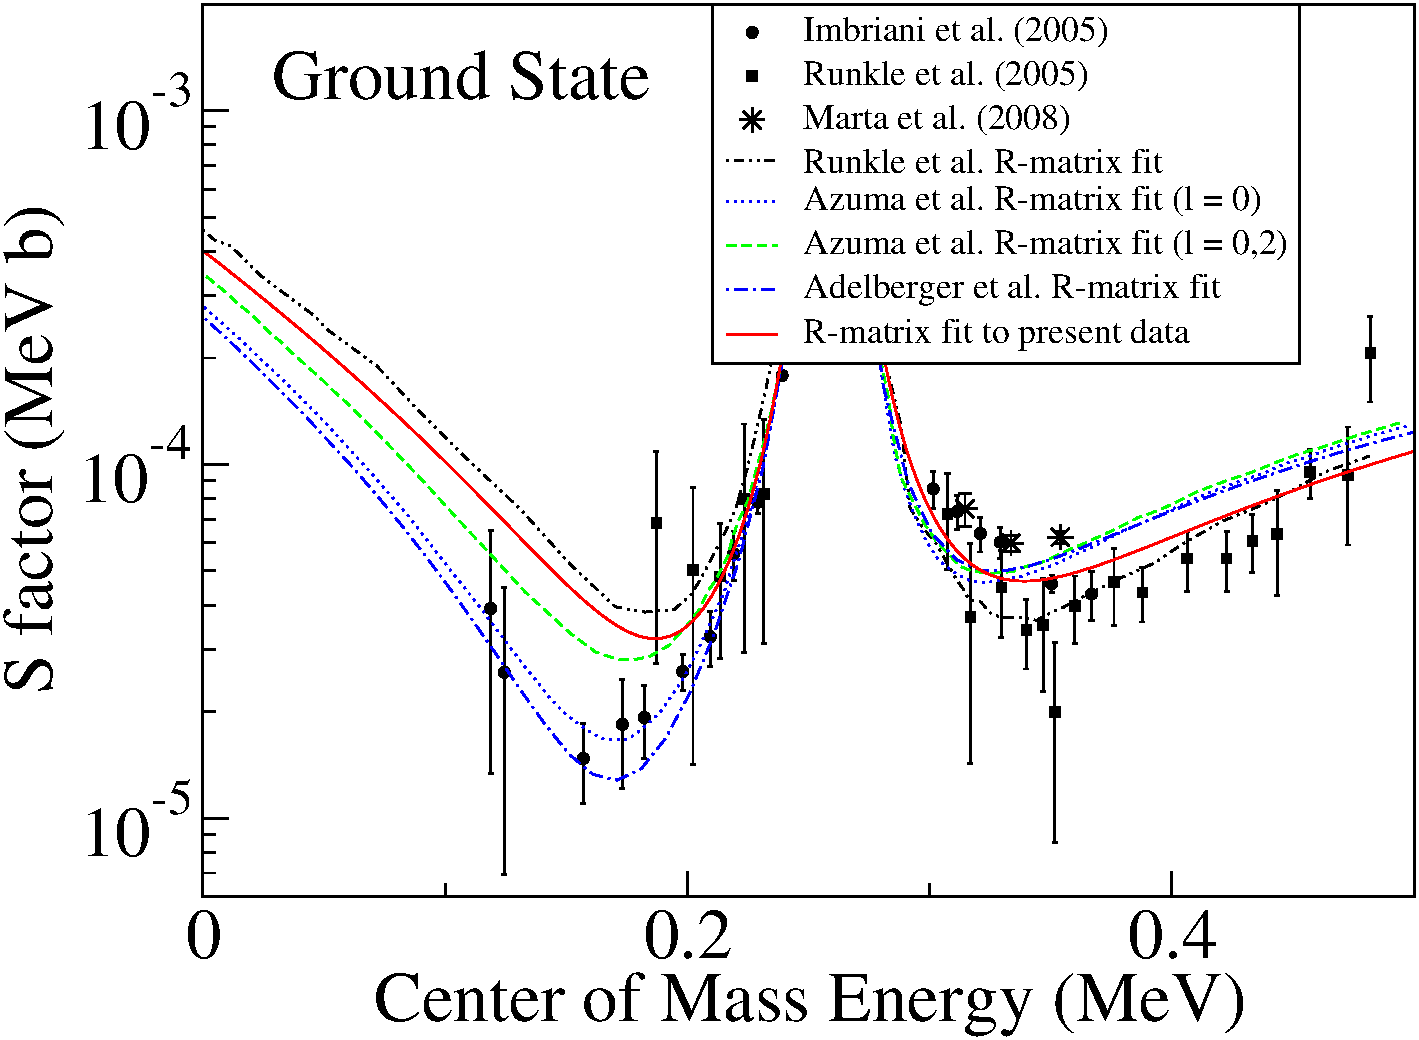
\includegraphics[width=\linewidth]{figures/qianSfactor.pdf}
\label{fig: QianRmatrix}
\caption{$R$-matrix extrapolation of the $S$-factor given in cite{Li2016}. The authors identified the major sources of uncertainty as the uncertainty as the DC/R$\rightarrow$gs primary transition, the DC/R$\rightarrow$6.17 MeV level primary transition, and the $\Gamma$ width of the 6.79 MeV state. Of these, the latter is the dominant term. This figure highlights the effects that these uncertainties have on low-energy extrapolations, varying by nearly a factor of two. }
\end{figure}

The Wagner \textit{et al.} study attempted to remedy this, providing an independent cross check of the ground state and 6.79 MeV capture transitions in the proton energy range of $E_{p}$ = 366–1289 keV, overlapping with the low-energy data sets. In the study, the authors found $S$-factors elevated significantly above those of any previous measurement for both of the transitions measured. Due to this, their results for the extrapolated $S(0)$ and contributions from the DC/R$\rightarrow$6.79 MeV transition agree with those from Li \textit{et al.}, but they are unable to draw conclusions about the ground state transition or any of the other, weaker transitions. Ultimately, this means that their results were unable to address any of the major uncertainties left plaguing the situation. 



\subsection{Lifetime}


As discussed, the $\Gamma$ width of the 6.79 MeV subthreshold state is the dominant uncertainty on the total $S$-factor at zero energy, as illustrated by Fig. \ref{fig: QianRmatrix}. The literature to date on the lifetimes/widths of the important levels in $\ce{^{15}O}$ are summarized in Table \ref{table: lifetimes}. Some of the values present in the table are those extracted as a fit parameter from $R$-matrix analyses, instead of experimental measurements cite{Schroder1987, Angulo2001, Fomicola2004, Runkle2005, Marta2008, Azuma2010, Adelberger2011}. By having a dominant term of the calculation be a floating fit parameter, accuracy and reliability in the extrapolations are lost. Therefore, determination of this quantity experimentally is critical. 


 \begin{table}[]
\begin{tabular}{lllll}
 &  &  &  &  \\
 &  &  &  &  \\
 &  &  &  &  \\
 &  &  &  & 
\end{tabular}
\label{table: lifetimes}
% copy qian's table  with the addition of TRIUMF (galinski) and Michelagnoli data
\caption{A summary of previous lifetime/width measurements for important states in $\ce{^{15}O}$. Currently a placeholder until I make the actual table.}
\end{table}

There are five measurements of the lifetime or width of the 6.79 MeV state ''directly'' cite{Bertone2001, Yamada2004, Schurmann2008, Galinski2014, Michelagnoli2016}, highlighted in red in Table \ref{table: lifetimes}, and they are unfortunately disparate in their extracted values and have relatively large errors. 

The first measurement was performed in 2001 by Bertone \textit{et al.}, using the Doppler Shift Attenuation Method (DSAM) to determine the lifetime of the state. This technique will be discussed in further detail later. The authors populated the state through resonant capture of protons in the $E_{p}$ = 278 keV state and observed the decaying $\gamma$-rays at three different angles. The measured lifetime for the 6.79 MeV state was determined to be $\tau = 1.60^{+0.75}_{-0.72}$ fs, corresponding to a width of $\Gamma = 0.41^{+0.34}_{-0.13}$ eV (determined by Equation \ref{eqn: width to lifetime}). 

At RIKEN, in 2004, Yamada \textit{et al.} performed a measurement of the radiative width via Coulomb Excitation experiment cite{Yamada2004} as an independent verification of the Bertone result. For this, $\ce{^{15}O}$ nuclei were produced by fragmentation of an $\ce{^{16}O}$ beam incident on a $\ce{^{9}Be}$ target and then inelastically scattered off of a thick lead target. The de-excitation $\gamma$-rays were detected with an array of NaI (Tl doped) scintillation detectors. In order to disentangle the 6.79 MeV peak of interest from the 6.86 Mev peak in their spectrum, the authors compared the experimentally obtained spectrum from with the results of a Monte Carlo simulation. Due to the poor energy resolution of the detector system, the authors ultimately had difficulty separating the peaks and only reported an upper bound on the width, $\Gamma = 0.95^{+0.60}_{-0.95}$ eV, and a corresponding lifetime of $\tau = 0.69 ^{+1.10}_{-0.69}$ fs. 

Four years later, Sch{\"u}rmann \textit{et al.} published a new measurement of the lifetime using the DSAM technique and an improved experimental setup cite{Schurmann2008}. This measurement used a single high-purity germanium (HPGe) detector on a rotating track and measuring at many more angles ranging from $40 - 116^{\deg}$, allowing for a check of asymmetries around the $90^{\deg}$ point and reducing systematic uncertainties from the use of different detectors. Similar to the Bertone measurement cite{Bertone2001}, the authors populated the state of interest via the resonance at $E_{p} = 278$ keV. In contrast to the Bertone result and similar to the Yamada work, the authors in this case could not recommend a finite value for the measured lifetime, obtaining a lifetime upper limit of $\tau < 0.77$ fs. 

In an attempt to provide another experimental technique for determining the lifetime, Galinski \textit{et al.} performed another DSAM measurement at the TRIUMF facility cite{Galinski2014}. The major difference this time, however, was that the reaction occurred in inverse kinematics (i.e. one where the heavier reaction input is accelerated towards the stationary, lighter one), emulating a result from over 50 years ago cite{Gill1968}. The $\ce{^{15}O}$ in this experiment were produced via the $\ce{^{3}He}(\ce{^{16}O},\alpha)\ce{^{15}O}$ reaction with a $\ce{^{3}He}$-implanted gold-foil and the de-excitation $\gamma$-rays were detected with a clover HPGe detector (a single detector containing four separate Ge crystals) and filtered in coincidence with the reaction product $\alpha$'s. The authors then determined the lifetime with a Bayesian line-shape analysis of the spectra and found a most probable lifetime of $\tau = 0$ fs and an upper limit given by experimental uncertainties of $\tau < 1.8$ fs with a 68.3\% confidence limit. The authors, however, acknowledge that their result was statistics limited.

The final measurement of this lifetime comes from an unpublished doctoral dissertation by Michelagnoli in 2013 cite{Michelagnoli2013}. Similar to Galinski \textit{et al.}, this measurement was done in inverse kinematics, with the $d(\ce{^{14}N},\ce{^{15}O})n$ reaction. The $\gamma$ rays from this measurement were detected with the state-of-the-art AGATA Demonstrator array using $\gamma$-ray tracking for precision angular data and a lineshape analysis of the data was performed by comparing with the results of a Monte Carlo simulation in the Geant4 software. This work also obtained only an upper-bound on the lifetime, $\tau < 1.0$ fs with a 68.3\% confidence limit. While this result is consistent with other literature values, it should nonetheless be taken with a grain of salt as it has not been peer-reviewed. 

In aggregate, these results are unsatisfactory, with an error that is still uncomfortably large. Particularly, the DSAM results (with the exception of Galinski cite{Galinski2014}) neglected the systematic uncertainties from the stopping power of the targets in their ultimate lifetime calculation. The forward kinematics reactions cite{Bertone2001, Schurmann2008} both used nitrogen-implanted tantalum-foils for the experiment (saturated to a composition of Ta$_{2}$N$_{3}$), but calculated the lifetimes assuming target densities and stopping powers equal to those of pure tantalum. However, in this lifetime range, the deceleration of the $\ce{^{15}O}$ nuclei occurs in the region where the nitrogen is present in the lattice. Specifically, this means that the presence of the nitrogen has a significant effect on the actual stopping power. According to the authors of the respective works, by using accurate densities and stopping powers the inferred lifetimes obtained in their works would have changed by 100\% cite{Bertone2001} and 2\% cite{Schurmann2008}, respectively. In both, the authors also contend that their calculations are appropriate because they used an identical method to calculate the lifetime of the 5.18 MeV state, agreeing with literature values.



\section{The Doppler Shift Attenuation Method for lifetime measurements}
\label{sec: dsam-intro}


Nuclear lifetimes are important observables to measure because they provide a link to understanding the strong nuclear force. They are necessary to determine the reduced transition probabilities which are one of the most important probes of nuclear structure and the forces governing the behavior of nuclei.The Doppler Shift Attenuation Method (DSAM) is a well characterized method for determining the lifetimes of excited nuclear states that decay via gamma emission in the range of 10$^{-11}$ - 10$^{-15}$ s cite{Alexander1968, Blaugrund1966}. The ranges where DSAM is applicable are compared with other common methods for determining nuclear lifetimes in Fig. \ref{fig: lifetimeRanges}. 


\begin{figure}
\label{fig: lifetimeRanges}
\caption{Ranges over which the different lifetime measuring techniques are valid.}
\end{figure}


The basic idea of DSAM is to produce an excited nucleus inside of a dense target in which the reaction product will decay. The de-excitation of the nucleus then takes place either while the nucleus is slowing down or after it stops, depending on the lifetime of the specific state and the stopping within the target. Then, as is true with the classical Doppler shift, the energy of the emitted $\gamma$-rays are shifted depending on their emission angle relative to the motion of their source, the decaying nucleus. Thus, $\gamma$'s emitted at different velocities during the slow-down and detected at given angles will have a spread of energies. Specifically, for a given nucleus decaying at a time $t$ with a speed of $v(t)$, the Doppler shifted energy of the gamma ray, $E_{\gamma}$, is 

\begin{equation}
E_{\gamma} = E_{0} \left(1 + \dfrac{v(t)}{c} \cos (\theta)   \right),
\label{eqn: doppler1}
\end{equation}

\noindent where $E_{0}$ is the energy of the decay for a nucleus at rest, $c$ is the speed of light, and $\theta$ is the lab angle between the momentum vectors of the decaying nucleus and gamma ray, respectively. A depiction of this scenario is given in Fig. \ref{fig: decay}.

\begin{figure}
\label{fig: decay}
\caption{A nuclear reaction showing the creation of an excited nucleus and subsequent decay , causing a Doppler shift in the measured energy of the $\gamma$ ray.}
\end{figure}


As the nuclear decay process is statistical in nature, the measured spectrum of gamma energies for a particular transition is a continuous distribution of energies from the unshifted, rest energy peak to the maximally Doppler shifted peak. As Equation \ref{eqn: doppler1} was specific to a single transition, it is necessary to consider the entire sample of decays measured. By defining the average velocity of all nuclei at the time of decay, $\overline{v}$, the initial velocity of all recoiling nuclei, $v_{0}$, and their ratio, $F(\tau)$, called the attenuation factor, it is possible to relate the behavior of the entire distribution to the lifetime of the state. This is 

\begin{equation}
E_{\gamma} = E_{0} \left(1 + F(\tau) \beta_{0} \cos (\theta)   \right),
\label{eqn: dopplerFull}
\end{equation}

\noindent where $\beta_{0} = v_{0}/c$ is the relativistic velocity factor. $F(\tau)$ therefore provides an analytical relation between the nuclear lifetime and the measured Doppler shift, given by Blaugrund in 1966 cite{Blaugrund1966} as

\begin{equation}
F(\tau) \beta_{0} = \dfrac{1}{\tau} \int_{0}^{\infty} \beta(t) \exp \left( \dfrac{t}{\tau} \right) dt,
\end{equation} 

\noindent where $\beta(t) = v(t)/c$ is the time dependent relativistic velocity factor. The devil, however, is in the details of calculating $\beta(t)$, since it is reliant on stopping powers of the nuclei in the target material, implying an accurate knowledge of the target composition and population pattern of the nucleus. In some cases the feeding is not well known and for nearly all cases, there is an estimated uncertainty in the assessment of stopping powers of materials to be at least 10\%.

It is important to note that the Doppler shift can either increase or decrease the energy of the measured $\gamma$ ray, depending on whether the emitted gamma ray is at forward or backward angles relative to the nucleus' motion. Fig. \ref{fig: dopplerShift} shows the Doppler effect on a measured $\gamma$ spectrum, shifting the energy according to the measured angle. It is evident that the lifetime of a particular excited state has a dramatic effect on the location and shape of this distribution, for the longer a specific lifetime is, the broader its measured distribution will be (and vice versa) while the shift in the centroid of the peak will be lower than that of short lifetimes where the nucleus has a relatively higher velocity upon decay. 

\begin{figure}
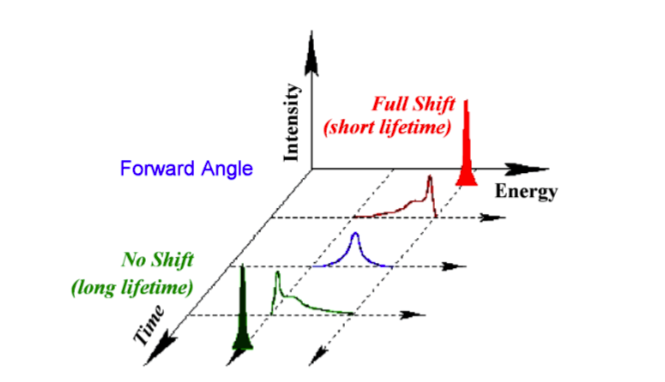
\includegraphics[width=\linewidth]{figures/dopplerEffects.png}
\label{fig: dopplerShift}
\caption{The effect of the nuclear lifetime on the measured gamma spectrum for a given experimental scenario cite{Schimpf2011}. In forward angles, the $\gamma$'s energy is shifted to higher values, while the the measured energy of the $\gamma$ is lower at backward angles, with the maximum shift in either direction coming when the $\gamma$ is emitted in a direction parallel to the motion of the decaying nucleus. A $\gamma$ emitted at $90^{\deg}$ is unshifted and unbroadened. }
\end{figure}

Therefore, by performing a lineshape analysis on the distribution of the measured $\gamma$'s and a mapping of the distribution's shift with angle one can determine the nuclear lifetime. The procedure for the Doppler shift determination is particularly straightforward. By plotting the resulting centroids measured for the gamma distribution vs the $\cos(\theta)$, one should obtain a straight line, the slope of which is the product $E_{0} \beta_{0} F(\tau)$. So, for a given experimental approach with the same reaction and targets, this slope and therefore attenuation factor should match. This was not the case for the Bertone \textit{et al.} and Sch{\"u}rmann \textit{et al.} works cite{Bertone2001, Schurmann2008}, where the authors used the same reaction on ostensibly the same targets and reached incongruous $F(\tau)$ values. 
 

\section{Thesis outline}
\label{sec: thesis outline}

In this dissertation, the results of a series of experiments and subsequent analyses performed to better understand the low energy behavior of the $^{14}$N$\left( p,\gamma \right) ^{15}$O will be presented. These include the measurement of the $^{14}$N$\left( p,\gamma \right) ^{15}$O reaction at the University of Notre Dame Nuclear Science Laboratory (NSL) and the Compact Accelerator System for Performing Astrophysical Research (CASPAR), located in the Sanford Underground Research Facility in the renovated Homestake Gold Mine in South Dakota, as well as a measurement of the lifetime of the 6.79 MeV level in $^{15}$O also at the NSL. 

An outline of the experimental techniques used in these measurements will be presented in Chapter \ref{chap: experiment}. There will be a brief overview of the equipment common to each of the measurements, with emphasis on the Van de Graaff accelerators and High-purity Germanium detectors used. Following this, the specific features of the different types of measurements and the facilities in which they were made will be presented. 

Chapters \ref{chap: data} - \ref{chap: lifetime} will present details on the different facets of the data reduction and analysis. The first of these, Chapter \ref{chap: data}, presents the data for $^{14}$N$\left( p,\gamma \right) ^{15}$O taken at the NSL and CASPAR while detailing the process by which the cross-section and astrophysical $S$-factor were extracted. Shifting focus, Chapter \ref{chap: simulation} will focus on the Monte Carlo code that was developed and used to simulate the lifetime of the states in $^{15}$O, presenting the results of these tests and displaying their ability to reproduce experimental cases. Finally, Chapter \ref{chap: lifetime} will present the actual Doppler shift analysis of the data done to extract the lifetime of the 6.79 MeV state in $^{15}$O. The validity of the method will be checked against other known levels populated in the reaction, like the states at 5.18 MeV and 6.17 MeV, respectively.

The cross-section information and newly measured lifetime will be utilized in a new $R$-matrix analysis of the $^{14}$N$\left( p,\gamma \right) ^{15}$O reaction, presented in Chapter \ref{chap: r-matrix}. The new constraints these data provide on the low-energy behavior of the extrapolated $S$-factor will be provided, alongside a description of their impact to relevant astrophysical quantities.

Finally, the contents of this dissertation will be summarized in Chapter \ref{chap: conclusions}. This will present an overview of the described measurements, analysis, respective impacts, and future outlook. 

% % uncomment the following lines,
% if using chapter-wise bibliography
%
% \bibliographystyle{ndnatbib}
% \bibliography{example}



%
% Chapter 2
%

%
% Modified by Megan Patnott
% Last Change: Jan 18, 2013
%
%%%%%%%%%%%%%%%%%%%%%%%%%%%%%%%%%%%%%%%%%%%%%%%%%%%%%%%%%%%%%%%%%%%%%%%%
%
% Modified by Bryce Frentz
% Last Change: 2018
%
%%%%%%%%%%%%%%%%%%%%%%%%%%%%%%%%%%%%%%%%%%%%%%%%%%%%%%%%%%%%%%%%%%%%%%%%
%
% Sample Notre Dame Thesis/Dissertation
% Using Donald Peterson's ndthesis classfile
%
% Written by Jeff Squyres and Don Peterson
%
% Provided by the Information Technology Committee of
%   the Graduate Student Union
%   http://www.gsu.nd.edu/
%
% Nothing in this document is serious except the format.  :-)
%
% If you have any suggestions, comments, questions, please send e-mail
% to: ndthesis@gsu.nd.edu
%
%%%%%%%%%%%%%%%%%%%%%%%%%%%%%%%%%%%%%%%%%%%%%%%%%%%%%%%%%%%%%%%%%%%%%%%%

%
% Chapter 2
%

\chapter{Experimental setup and procedures}
\label{chap: experiment}

\section{Introduction}

This set of data was taken over the course of five* separate experiments. The first occurred at the University of Notre Dame's Nuclear Science Laboratory (NSL) in January of 2018 and covered the proton energy range of E$_{p}$ = 800 - 1200 keV. The experiment was then continued at the Compact Accelerator System for Performing Nuclear Astrophysics (CASPAR) facility at the Sanford Underground Research Facility located in Lead, South Dakota in three increments: February 2018, May 2018, and August / September 2018. These measurements covered the energy range from E$_{p}$ = 270 - 1200 keV, in order to measure the $^{14}$N$\left( p,\gamma \right) ^{15}$O reaction cross-section to compare the performance of the CASPAR facility to an above-ground laboratory. Finally, in MONTH TIME DATE THING, the final experiment was completed at the NSL, focusing on obtaining the lifetime of the 6793 keV state in $^{15}$O.

\section{Accelerators, beamline, and high-purity Germanium detectors}
\label{sec: accelerators, beamline, and detectors}



\subsection{Van de Graaff accelerators}

\subsection{Ion sources}

\subsection{Beamline}



\section{High-purity Germanium detectors}
\label{sec: HPGe detectors}


\section{Cross-section measurements}
\label{sec: nsl experiment}


\section{Lifetime measurement}
\label{sec: caspar experiment}




% % uncomment the following lines,
% if using chapter-wise bibliography
%
% \bibliographystyle{ndnatbib}
% \bibliography{example}


%
% Chapter 3
%

%
% Modified by Megan Patnott
% Last Change: Jan 18, 2013
%
%%%%%%%%%%%%%%%%%%%%%%%%%%%%%%%%%%%%%%%%%%%%%%%%%%%%%%%%%%%%%%%%%%%%%%%%
%
% Modified by Bryce Frentz
% Last Change: 2018
%
%%%%%%%%%%%%%%%%%%%%%%%%%%%%%%%%%%%%%%%%%%%%%%%%%%%%%%%%%%%%%%%%%%%%%%%%
%
% Sample Notre Dame Thesis/Dissertation
% Using Donald Peterson's ndthesis classfile
%
% Written by Jeff Squyres and Don Peterson
%
% Provided by the Information Technology Committee of
%   the Graduate Student Union
%   http://www.gsu.nd.edu/
%
% Nothing in this document is serious except the format.  :-)
%
% If you have any suggestions, comments, questions, please send e-mail
% to: ndthesis@gsu.nd.edu
%
%%%%%%%%%%%%%%%%%%%%%%%%%%%%%%%%%%%%%%%%%%%%%%%%%%%%%%%%%%%%%%%%%%%%%%%%

%
% Chapter 3
%

\chapter{Cross section data Reduction and analysis}
\label{chap: data}

\section{Introduction}

$^{14}$N$\left( p,\gamma \right) ^{15}$O\\

\section{Energy calibration}
\label{sec: energy calibration}

\section{Efficiency}
\label{sec: efficiency}

\subsection{Total efficiency}

\subsection{Full energy peak efficiency}


\section{Summing corrections}
\label{sec: summing}

\section{Target characterization}
\label{sec: target}

\section{Cross-section determination}
\label{sec: cross-section}





% % uncomment the following lines,
% if using chapter-wise bibliography
%
% \bibliographystyle{ndnatbib}
% \bibliography{example}


%
% Chapter 4
%

%
% Modified by Megan Patnott
% Last Change: Jan 18, 2013
%
%%%%%%%%%%%%%%%%%%%%%%%%%%%%%%%%%%%%%%%%%%%%%%%%%%%%%%%%%%%%%%%%%%%%%%%%
%
% Modified by Sameer Vijay
% Last Change: Tue Jul 26 2005 13:00 CEST
%
%%%%%%%%%%%%%%%%%%%%%%%%%%%%%%%%%%%%%%%%%%%%%%%%%%%%%%%%%%%%%%%%%%%%%%%%
%
% Sample Notre Dame Thesis/Dissertation
% Using Donald Peterson's ndthesis classfile
%
% Written by Jeff Squyres and Don Peterson
%
% Provided by the Information Technology Committee of
%   the Graduate Student Union
%   http://www.gsu.nd.edu/
%
% Nothing in this document is serious except the format.  :-)
%
% If you have any suggestions, comments, questions, please send e-mail
% to: ndthesis@gsu.nd.edu
%
%%%%%%%%%%%%%%%%%%%%%%%%%%%%%%%%%%%%%%%%%%%%%%%%%%%%%%%%%%%%%%%%%%%%%%%%


%
% Chapter 4
%

\chapter{Monte Carlo simulations for lifetime measurements with DSAM}
\label{chap: simulation}

\section{Simulations with the Geant4 package}
\label{sec: geant}

\section{Determining a nuclear lifetime}
\label{sec: lifetime simulation}

% % uncomment the following lines,
% if using chapter-wise bibliography
%
% \bibliographystyle{ndnatbib}
% \bibliography{example}


%
% Chapter 5
%

%
% Modified by Megan Patnott
% Last Change: Jan 18, 2013
%
%%%%%%%%%%%%%%%%%%%%%%%%%%%%%%%%%%%%%%%%%%%%%%%%%%%%%%%%%%%%%%%%%%%%%%%%
%
% Modified by Sameer Vijay
% Last Change: Tue Jul 26 2005 13:00 CEST
%
%%%%%%%%%%%%%%%%%%%%%%%%%%%%%%%%%%%%%%%%%%%%%%%%%%%%%%%%%%%%%%%%%%%%%%%%
%
% Sample Notre Dame Thesis/Dissertation
% Using Donald Peterson's ndthesis classfile
%
% Written by Jeff Squyres and Don Peterson
%
% Provided by the Information Technology Committee of
%   the Graduate Student Union
%   http://www.gsu.nd.edu/
%
% Nothing in this document is serious except the format.  :-)
%
% If you have any suggestions, comments, questions, please send e-mail
% to: ndthesis@gsu.nd.edu
%
%%%%%%%%%%%%%%%%%%%%%%%%%%%%%%%%%%%%%%%%%%%%%%%%%%%%%%%%%%%%%%%%%%%%%%%%


%
% Chapter 5
%

\chapter{The lifetime of the 6.79 MeV state in $^{15}$O}
\label{chap: lifetime}

\section{Data analysis}
\label{sec: lifetime analysis}


\subsection{Lifetime of \textbf{ANOTHER STATE, 6.17 MeV maybe}}

\subsection{Lifetime of the 6.79 MeV state in $^{15}$O}



% % uncomment the following lines,
% if using chapter-wise bibliography
%
% \bibliographystyle{ndnatbib}
% \bibliography{example}


%
% Chapter 6
%

%
% Modified by Megan Patnott
% Last Change: Jan 18, 2013
%
%%%%%%%%%%%%%%%%%%%%%%%%%%%%%%%%%%%%%%%%%%%%%%%%%%%%%%%%%%%%%%%%%%%%%%%%
%
% Modified by Sameer Vijay
% Last Change: Tue Jul 26 2005 13:00 CEST
%
%%%%%%%%%%%%%%%%%%%%%%%%%%%%%%%%%%%%%%%%%%%%%%%%%%%%%%%%%%%%%%%%%%%%%%%%
%
% Sample Notre Dame Thesis/Dissertation
% Using Donald Peterson's ndthesis classfile
%
% Written by Jeff Squyres and Don Peterson
%
% Provided by the Information Technology Committee of
%   the Graduate Student Union
%   http://www.gsu.nd.edu/
%
% Nothing in this document is serious except the format.  :-)
%
% If you have any suggestions, comments, questions, please send e-mail
% to: ndthesis@gsu.nd.edu
%
%%%%%%%%%%%%%%%%%%%%%%%%%%%%%%%%%%%%%%%%%%%%%%%%%%%%%%%%%%%%%%%%%%%%%%%%


%
% Chapter 6
%

\chapter{R-matrix analysis}
\label{chap: r-matrix}

\section{Fits to the capture data}
\label{sec: capture fit}



\section{Inclusion of the new lifetime}
\label{sec: lifetime fit}

% % uncomment the following lines,
% if using chapter-wise bibliography
%
% \bibliographystyle{ndnatbib}
% \bibliography{example}


%
% Chapter 7
%

%
% Modified by Megan Patnott
% Last Change: Jan 18, 2013
%
%%%%%%%%%%%%%%%%%%%%%%%%%%%%%%%%%%%%%%%%%%%%%%%%%%%%%%%%%%%%%%%%%%%%%%%%
%
% Modified by Sameer Vijay
% Last Change: Tue Jul 26 2005 13:00 CEST
%
%%%%%%%%%%%%%%%%%%%%%%%%%%%%%%%%%%%%%%%%%%%%%%%%%%%%%%%%%%%%%%%%%%%%%%%%
%
% Sample Notre Dame Thesis/Dissertation
% Using Donald Peterson's ndthesis classfile
%
% Written by Jeff Squyres and Don Peterson
%
% Provided by the Information Technology Committee of
%   the Graduate Student Union
%   http://www.gsu.nd.edu/
%
% Nothing in this document is serious except the format.  :-)
%
% If you have any suggestions, comments, questions, please send e-mail
% to: ndthesis@gsu.nd.edu
%
%%%%%%%%%%%%%%%%%%%%%%%%%%%%%%%%%%%%%%%%%%%%%%%%%%%%%%%%%%%%%%%%%%%%%%%%


%
% Chapter 7
%

\chapter{Results and conclusions}
\label{chap: conclusions}


% % uncomment the following lines,
% if using chapter-wise bibliography
%
% \bibliographystyle{ndnatbib}
% \bibliography{example}



%
% Appendix (optional)
%

\appendix

%
% Modified by Sameer Vijay
% Last Change: Wed Jul 27 2005 13:00 CEST
%
%%%%%%%%%%%%%%%%%%%%%%%%%%%%%%%%%%%%%%%%%%%%%%%%%%%%%%%%%%%%%%%%%%%%%%%%
%
% Sample Notre Dame Thesis/Dissertation
% Using Donald Peterson's ndthesis classfile
%
% Written by Jeff Squyres and Don Peterson
%
% Provided by the Information Technology Committee of
%   the Graduate Student Union
%   http://www.gsu.nd.edu/
%
% Nothing in this document is serious except the format.  :-)
%
% If you have any suggestions, comments, questions, please send e-mail
% to: ndthesis@gsu.nd.edu
%
%%%%%%%%%%%%%%%%%%%%%%%%%%%%%%%%%%%%%%%%%%%%%%%%%%%%%%%%%%%%%%%%%%%%%%%%

%%%%%%%%%%%%%%%%%%%%%%%%%%%%%%%%%%%%%%%%%%%%%%%%%%%%%%%%%%%%%%%%%%%%%%%%
%
% Appendix
%
%%%%%%%%%%%%%%%%%%%%%%%%%%%%%%%%%%%%%%%%%%%%%%%%%%%%%%%%%%%%%%%%%%%%%%%%

\chapter{GNU GENERALISMS}

\section{Definitions}

Several definitions are presented in Table~\ref{tbl:defs} to show both
how to do rotated, line-spanning tables, as well as to define some
commonly used Gnu terms.

\begin{landscape}
\begin{table}
\centering
\caption{Commonly used \NoCaseChange{Gnu} Terms \label{tbl:defs}}
\begin{tabular}{lp{5in}}
\toprule
Term & \multicolumn{1}{c}{Definition} \\
\midrule
Gnu & Small furry animal that is related to the squirrel 
(although they won't admit it). \\
LoG & Abbreviation for the ``Leader of Gnus''.  See
Chapter~\ref{chap:golfing}. \\
Twizzlers & Red, twisty candy that is among the most favorite of Gnu
foods.  Gnus frequently appear overly cute and friendly to humans
bearing twizzler packages.  This is known as ``trolling for twizzlers''
among the Gnus. \\
\bottomrule
\end{tabular}
\end{table}
\end{landscape}

Finally, Table~\ref{tbl:rotated-rankings} shows the top ten Gnus from
Table~\ref{tbl:votes} ranked in order by their aggregate score (along
with some of the raters' comments).  This follows a long-standing Gnu
tradition of self-improvement through public announcement of score
(which some associate with military
origins~\citep{galmira98:_gnus_milit}).  Indeed, this very table has
been observed in the Gnu lodge where it was posted for peer review
\citep{gairley2000}.


\begin{landscape}
% set the caption width to be somewhat short since our table is narrow
% Notice the special commands that we use here to get the right line in the
% table.  Using \hrule is *not* the Right Thing to do here -- use
% \cmidrule.  We use the LaTeX \newcommand simply for convenience.
%
% The longtable package does some nasty voodoo to make \hline work OK.
% So on with the goods
\setlength\LTcapwidth{4.5in}
\begin{longtable}{lcp{4.5in}}
% Note that after the caption line we remove 2em worth of space but in the
% longtable of Chapter 2 we only remove 1em.  This is because a normal 
% \toprule has no space above it, but here we are using cmidrule which does 
% have padding above which we must account for.
  \caption{Top Ten \NoCaseChange{Gnus} From
    Table~\NoCaseChange{\ref{tbl:votes}} With Reviewer Comments.
    \NoCaseChange{Gnus} are Listed Below in Alphabetic Order.
    \label{tbl:rotated-rankings} }\\
  \toprule
  Candidate & Aggregate score & \multicolumn{1}{c}{Reviewer Comments}\\
  \midrule
\endfirsthead
  \caption[]{{\em Continued}} \\  % Just like in Chp. 2
  \midrule
  Candidate & Aggregate score & \multicolumn{1}{c}{Reviewer Comments}\\
  \midrule
\endhead
\endfoot
  \bottomrule
\endlastfoot
George & 7.6 & George is an excellent candidate for the LoG.
  Slightly low C, but hopefully, this 7.6 will be high enough! \\
Glen & 7.2 & A little weak on AM and Fr, but good scores overall.  One
  or two more years of experience should be enough. \\
Goldie & 7.0 & Dismal score in Fr; suspect it had something to do with
  strenuous weight loss program this past year. \\
Gillian & 6.9 & Excellent C, but a little shabby on the Fu.  Suggest
  more roughage. \\
Gibby & 6.9 & Reasonable scores, but need to work on Fr.  Gibby is
  definitely not a morning Gnu. \\ 
Genaveve & 6.5 & Very low Fr; perhaps more coffee?  Suggest practicing
  ``cute faces'' in the mirror several hours per day.  \\
Giovani & 6.2 & Very low Fr; suspect hanging out with Genaveve too
  much. \\
Gina & 6.2 & Mediochre Fu, somewhat low AM.  Perhaps a future in
  marketing or advertising? \\
Garrick & 6.2 & Fairly low AM.  Fu could be better as well; buy a
  comb.  And a mirror.  Immediately.  \\
Gardenia & 6.0 & Dismal AM; very low Fu.  Seems to care more about
  meeting agendas than personal appearance. \\
\end{longtable}
\end{landscape}


% % uncomment the following lines,
% if using chapter-wise bibliography
%
% \bibliographystyle{ndnatbib}
% \bibliography{example}



%
% Back stuff
%

 \backmatter
 \bibliographystyle{nddiss2e_edited} % The standard abbrvnat style should be acceptable. Also provided with both the advanced and standard
% \bibliography{example}       % distributions are nddiss2e and nddiss2enoarticletitles style options.
 \bibliography{dissertationBibliography}


\end{document}

% End of ``example.tex''
